% TEXINPUTS=.:$HOME/git/bvtex: latexmk  -pdf <main>.tex
\documentclass[xcolor=dvipsnames]{beamer}

\input{defaults}
\input{beamer/preamble}

\setbeamertemplate{navigation symbols}{}
% \setbeamertemplate{background}[grid][step=1cm]

\usepackage{siunitx}
\usepackage{xmpmulti}
\usepackage[export]{adjustbox}

\usepackage[outline]{contour}
\usepackage{tikz}
\usetikzlibrary{shapes.geometric, arrows}
\usetikzlibrary{positioning}

\definecolor{bvtitlecolor}{rgb}{0.98, 0.92, 0.84}
\definecolor{bvoutline}{rgb}{0.1, 0.1, 0.1}

\renewcommand{\bvtitleauthor}{Brett Viren}
\renewcommand{\bvtit}{LARF 2D}
\renewcommand{\bvtitle}{\LARGE LARF Parallel Wires\\Mimic a 2D Calculation\\\textbf{Notes and Problems}}
\renewcommand{\bvevent}{notes}
\renewcommand{\bvbeamerbackground}{}

\newcommand{\microboone}{MicroBooNE\xspace}


\begin{document}
\input{beamer/title.tex}

\begin{frame}
  \frametitle{Parallel Wires - Parameters}
  Try to match 2D calculation with 3D, parallel wires.
  \begin{description}
  \item[planes] 13 wires in each plane, all parallel.
  \item[wires] 3mm pitch and gap, 0.15mm radius, 30mm length, 1.5mm mesh.
  \item[cathode] -500 V (and ground) planes at +20 mm (-20 mm), 2.5mm mesh.
  \item[precision] Double the BEM Gaussian quadrature orders.
  \item[resolution] raster grid at 500x10x500.
  \end{description}
\end{frame}

\begin{frame}
  \frametitle{Parallel Wires - Weighting Potentials}
  \begin{columns}
    \begin{column}{0.3\textwidth}
      \begin{center}
        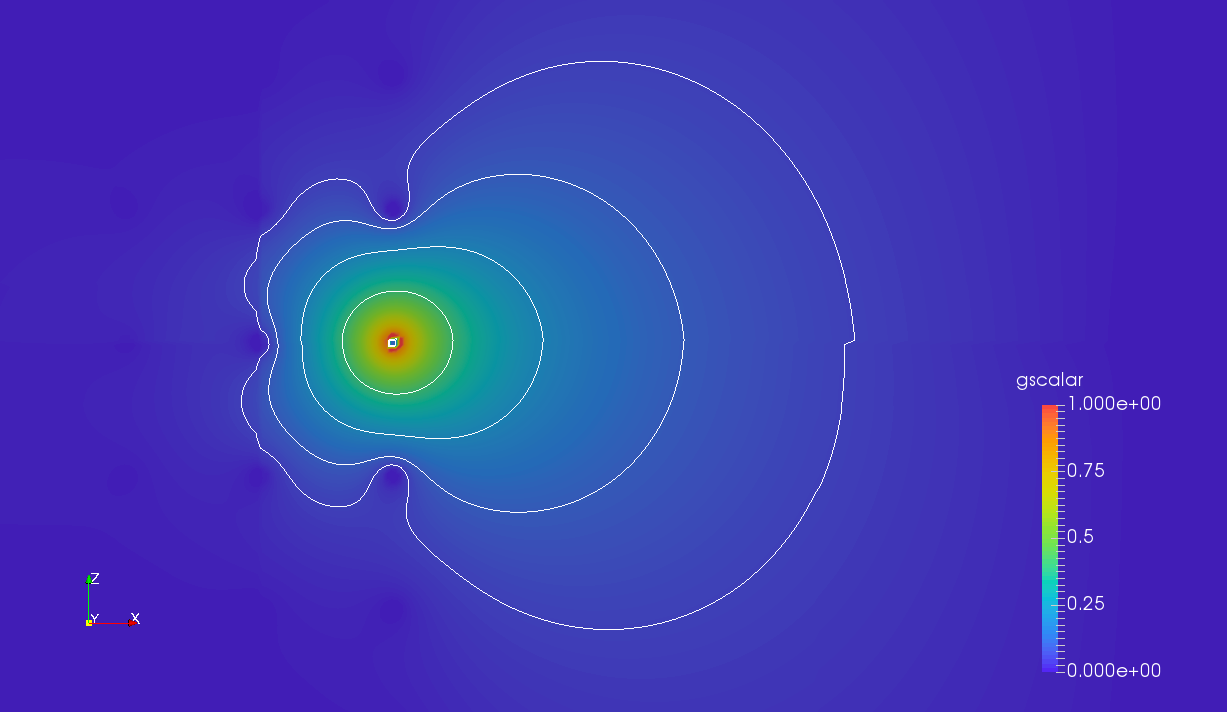
\includegraphics[height=2cm]{twodee-fine-u7.png}

        \scriptsize U plane
      \end{center}
    \end{column}
    \begin{column}{0.3\textwidth}
      \begin{center}
        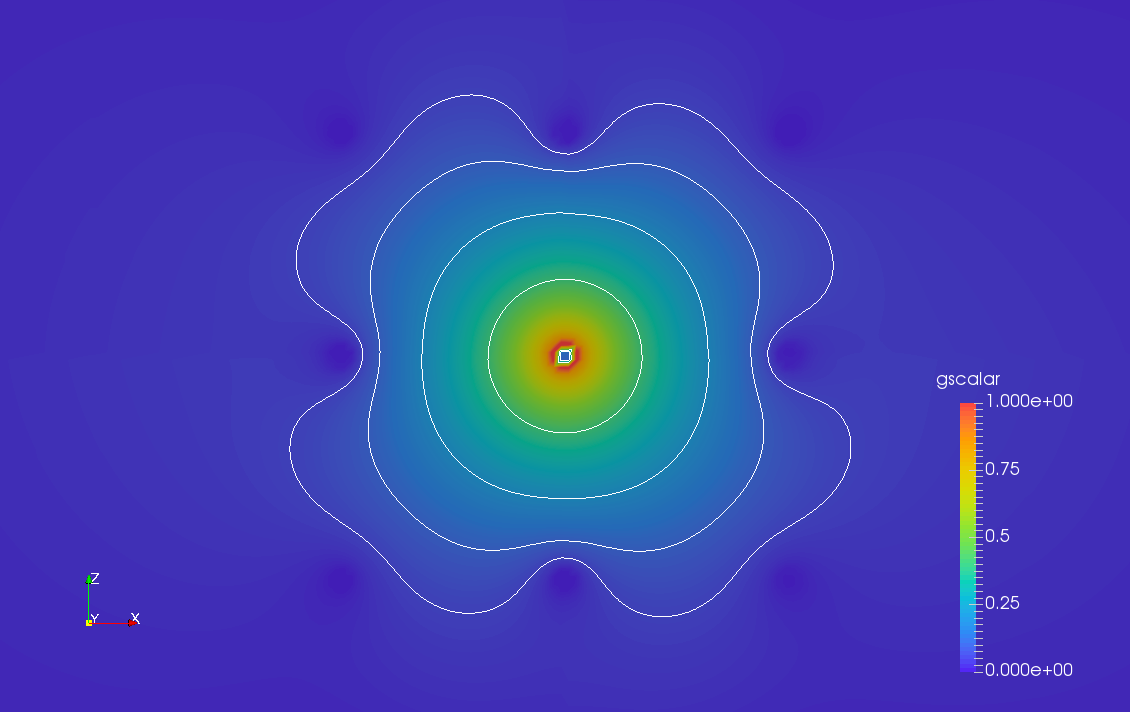
\includegraphics[height=2cm]{twodee-fine-v7.png}
        
        \scriptsize V plane
      \end{center}
    \end{column}
    \begin{column}{0.3\textwidth}
      \begin{center}
        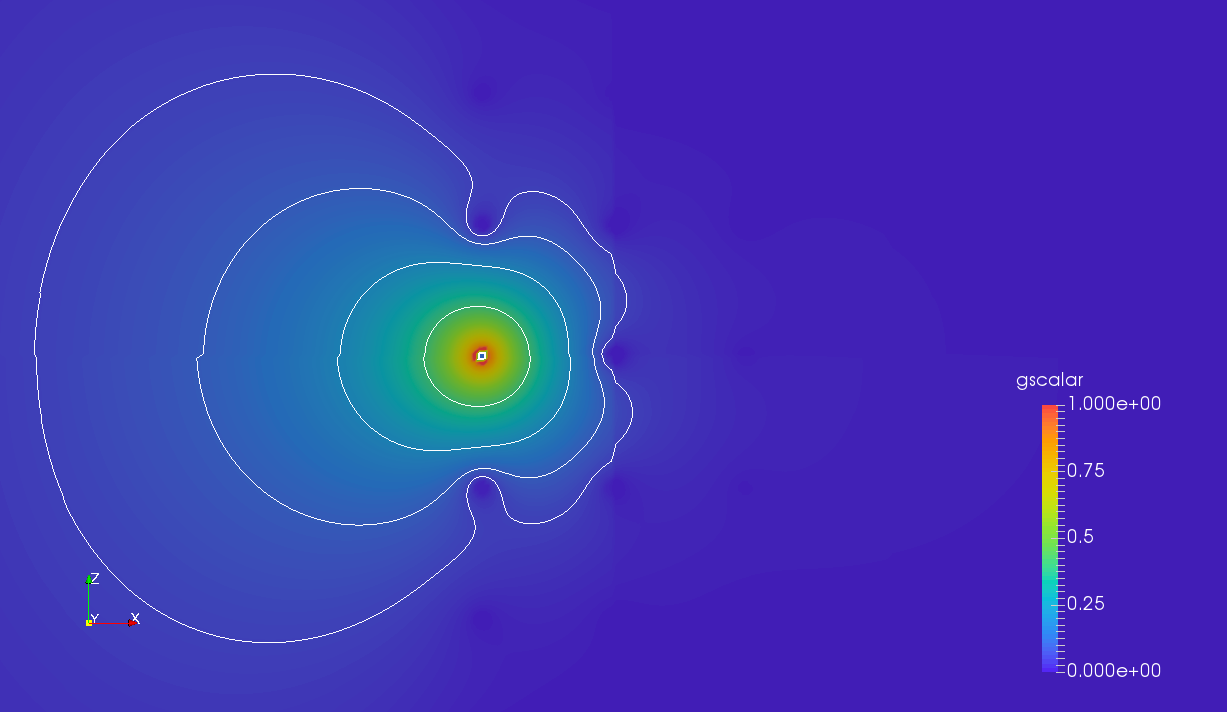
\includegraphics[height=2cm]{twodee-fine-w7.png}

        \scriptsize W plane
      \end{center}
    \end{column}
  \end{columns}

  \begin{itemize}\footnotesize
  \item X-Z slice through Y=0.
  \item Color shows weighting potential: 0-100\%.
  \item Lines: 5\%, 10\%, 20\%, 40\% weights.
  \item Gaussian quadrature imprecision visible in some jaggy contous lines.
  \item Small spatial fluctuations near wires, but somewhat obscured.
    \begin{itemize}
    \item Note: inside wire is $\sim$0V, square shape is pixelization.
    \end{itemize}
  \end{itemize}

\end{frame}


\begin{frame}
  \frametitle{Parallel Wires - Drift Potential}
  \begin{center}
    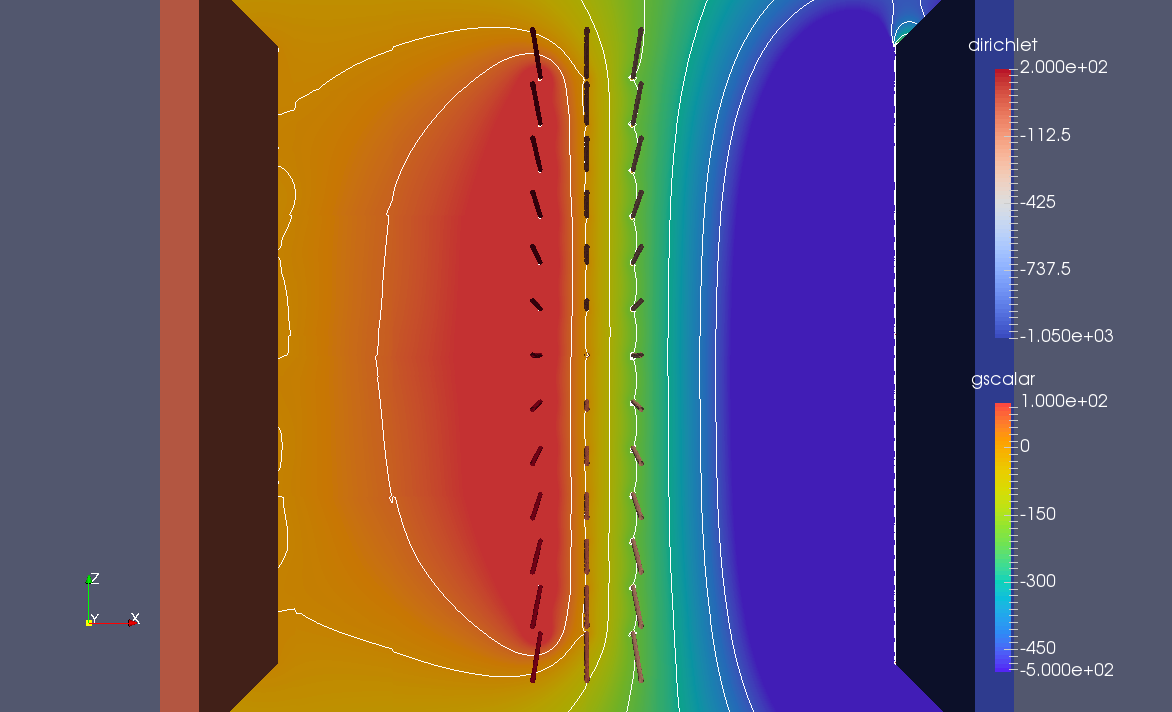
\includegraphics[width=0.7\textwidth]{twodee-fine-drift-plan.png}
  \end{center}
  \begin{itemize}\footnotesize
  \item X-Z slice through Y=0, looking down Y-axis.
  \item Equipotential lines: 50, 0, -100, -200, -300, -400, -450V.
  \end{itemize}
\end{frame}
\begin{frame}
  \frametitle{Parallel Wires - Drift Potential}
  \begin{center}
    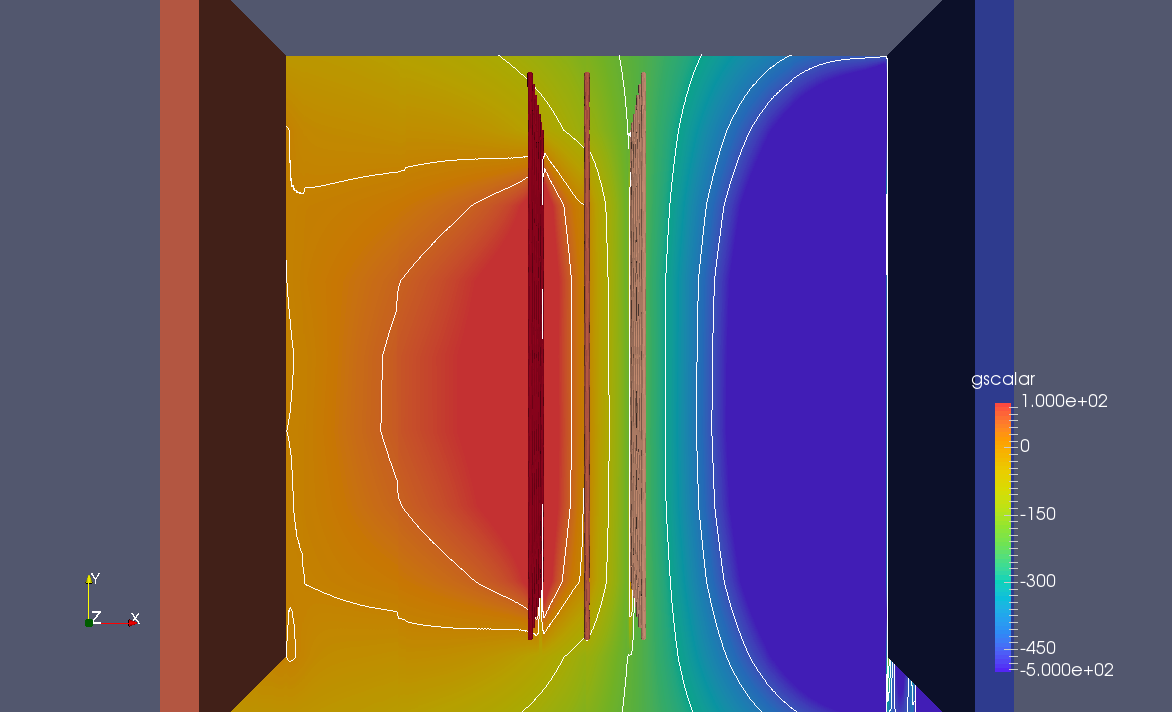
\includegraphics[width=0.7\textwidth]{twodee-fine-drift-side.png}
  \end{center}
  \begin{itemize}\footnotesize
  \item X-Z slice through Y=0, side view.
  \item More divergence that wanted for emulating an infinite plane.
  \item Off-by-one-half-pixel between mesh and field, just drawing artifact (I think).
  \end{itemize}
\end{frame}

\begin{frame}
  \frametitle{Parallel Wires - Drift Potential}
  \begin{center}
    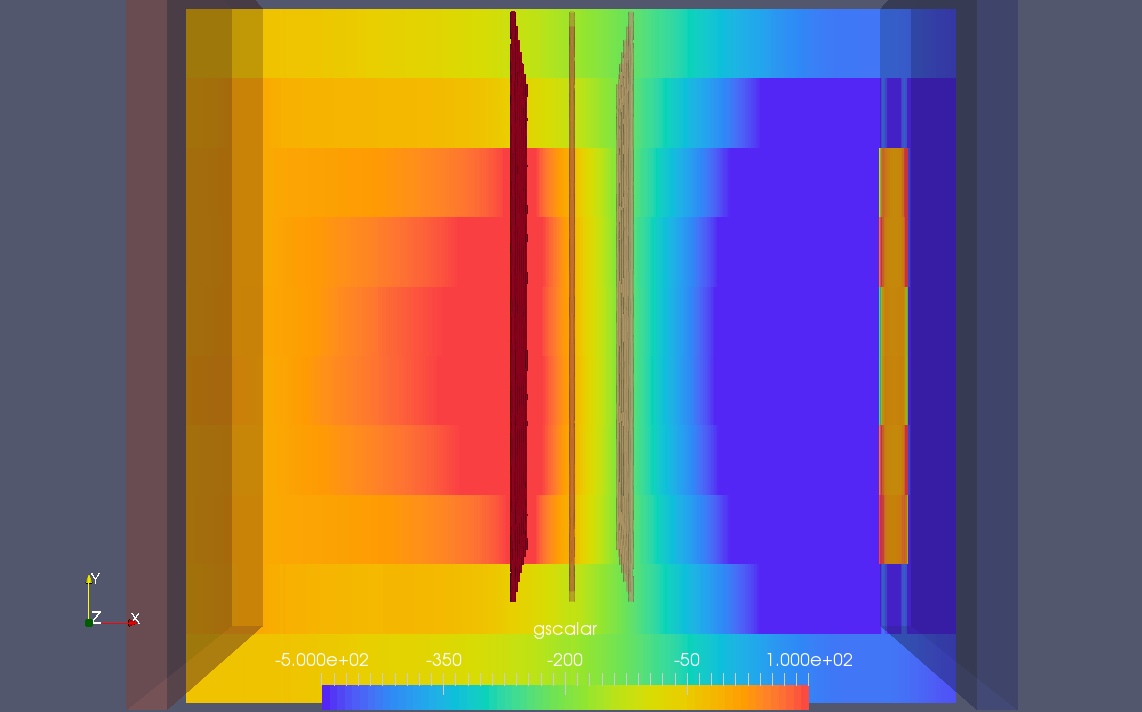
\includegraphics[width=0.7\textwidth]{twodee-fine-drift-field-side.png}
  \end{center}
  \begin{itemize}\footnotesize
  \item Same but actual voxels size.
  \end{itemize}
\end{frame}

\begin{frame}
  \frametitle{Parallel Wires - Steps}
  \begin{center}
    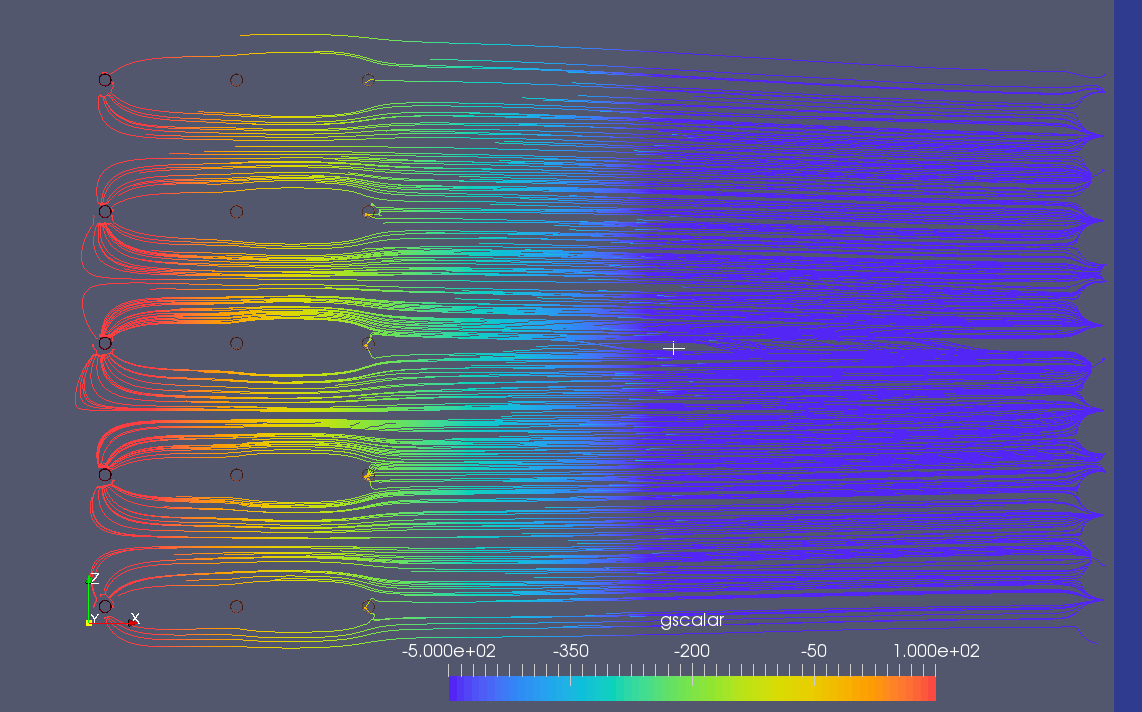
\includegraphics[width=0.7\textwidth]{twodee-fine-drift-steps-plan.png}    
  \end{center}
  \begin{itemize}\footnotesize
  \item Uses ParaView's build in R-K stepper, color still shows potential.
  \item This is looking down the Y-axis, but actually 3D steps.
  \item Each stepping goes for fixed length and then quits, tracks
    terminating around the cyan, explained next.
  \end{itemize}
\end{frame}

\begin{frame}
  \frametitle{Parallel Wires - Steps}
  \begin{center}
    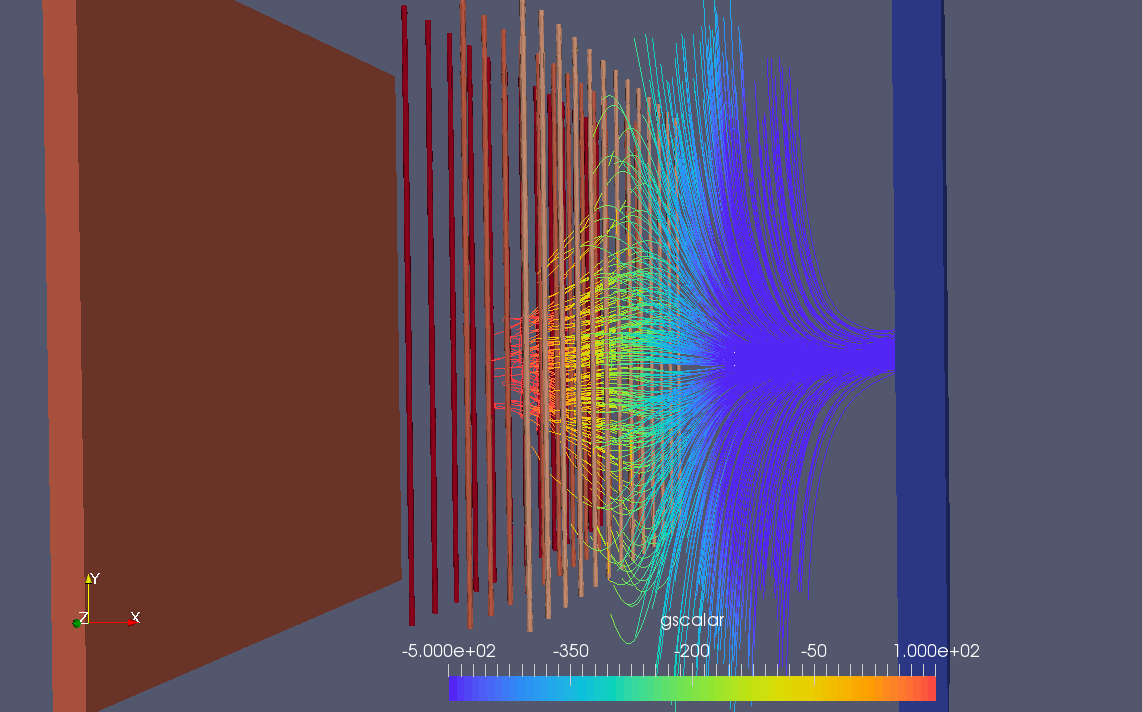
\includegraphics[width=0.7\textwidth]{twodee-fine-drift-steps-side.png}    
  \end{center}
  \begin{itemize}\footnotesize
  \item Side view of same scene.
  \item Clear effect of divergent stepping field.  Any off-center tracks quickly diverge.
  \end{itemize}
\end{frame}

\begin{frame}
  \frametitle{Problem is Non-square Voxels}
  \begin{columns}
    \begin{column}{0.5\textwidth}
      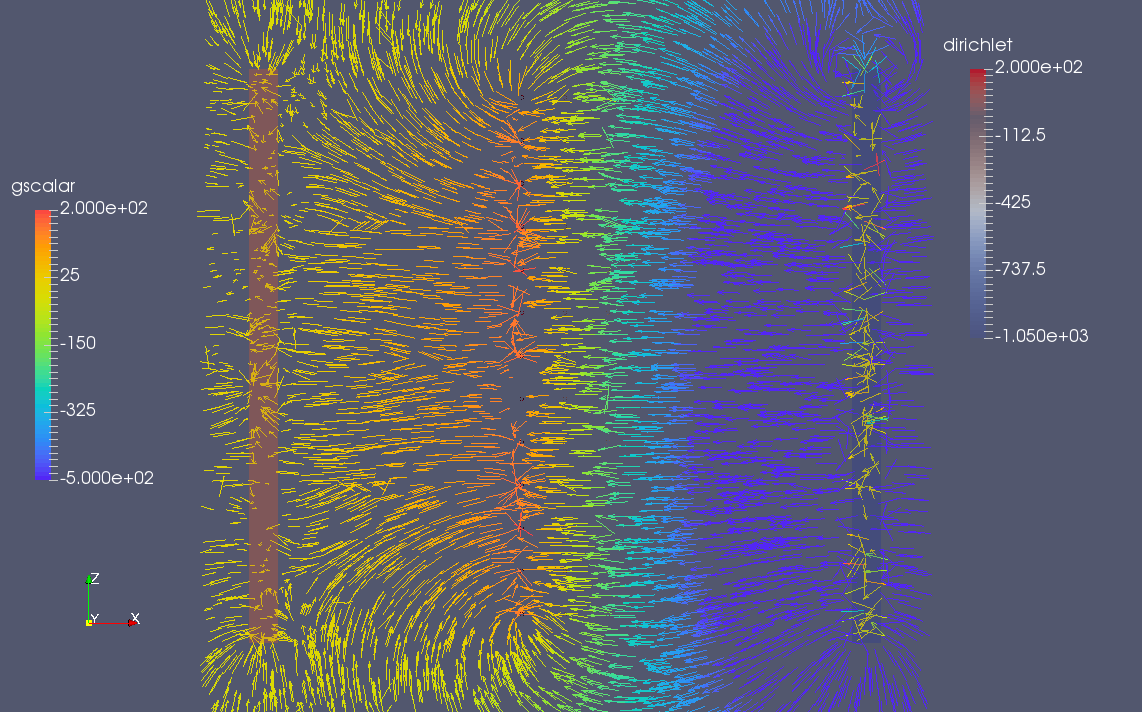
\includegraphics[width=\textwidth]{twodee-fine-arrows-plan.png}      
    \end{column}
    \begin{column}{0.5\textwidth}
      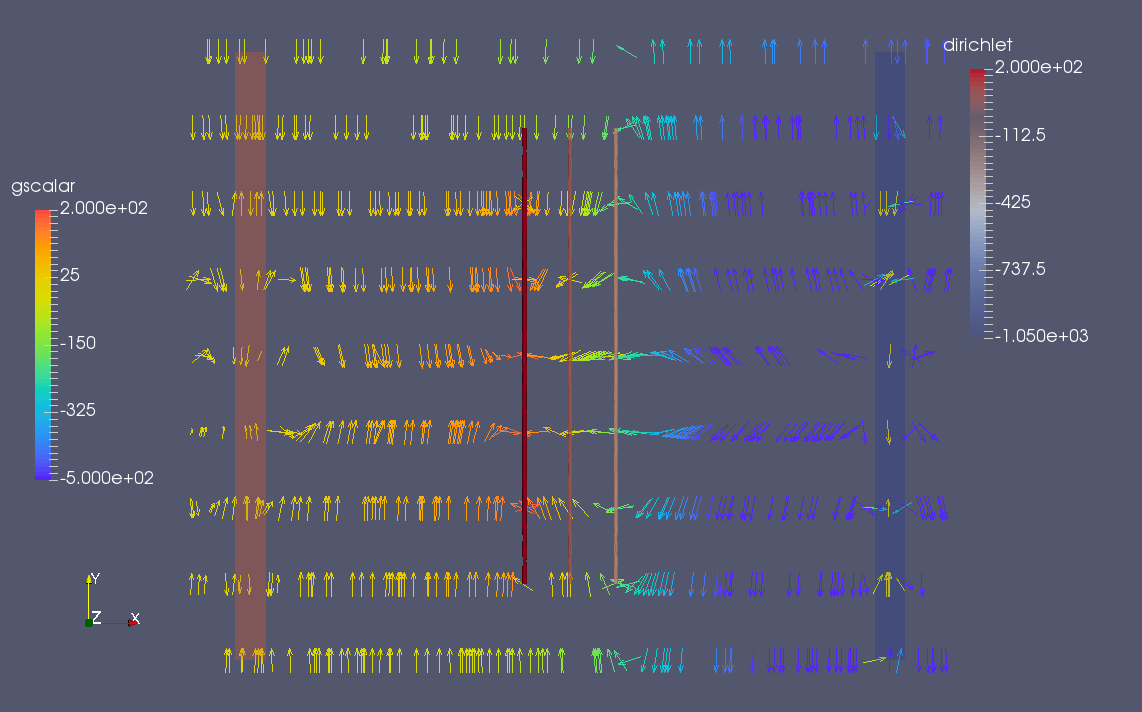
\includegraphics[width=\textwidth]{twodee-fine-arrows-side.png}      
    \end{column}
  \end{columns}
  \footnotesize
  \begin{itemize}
  \item X-Z and Y-Z slices with vector field drawn.  Clearly vector
    field in Y direction is wrong given potential.
  \item Potential pixels are 0.1mm in X and Z, 5mm in Y.  This is
    probably not being taken into account in the gradient!
  \end{itemize}
\end{frame}

\begin{frame}
  \frametitle{After gradient fix - vector field}
  \begin{columns}
    \begin{column}{0.5\textwidth}
      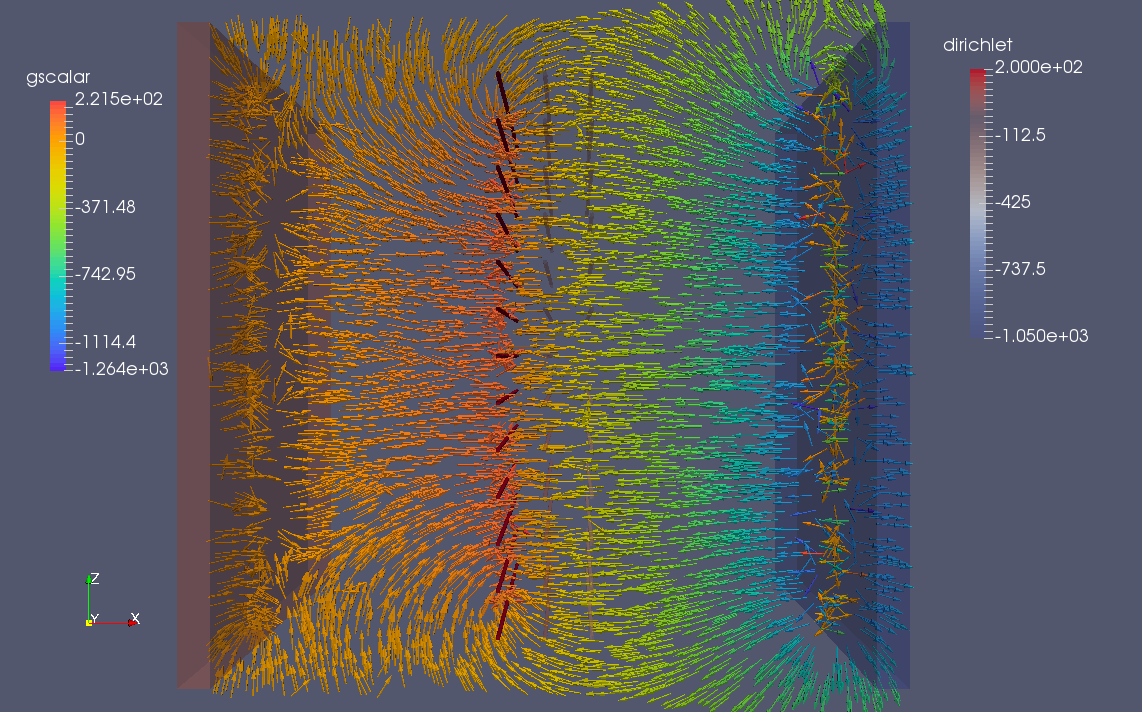
\includegraphics[width=\textwidth]{twodee-fine-arrows-plan-fixgrad.png}      
    \end{column}
    \begin{column}{0.5\textwidth}
      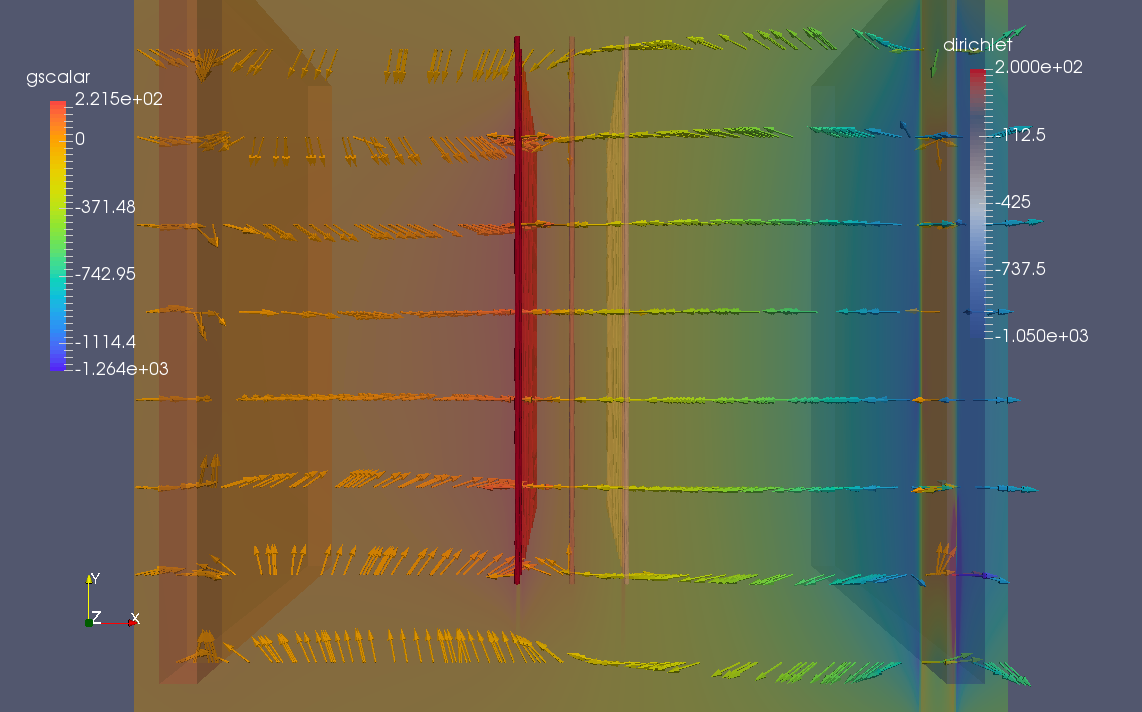
\includegraphics[width=\textwidth]{twodee-fine-arrows-side-fixgrad.png}      
    \end{column}
  \end{columns}
  \footnotesize
  \begin{itemize}
  \item Much more reasonable looking vectors.
  \item Still some divergence toward top/bottom.
  \end{itemize}
\end{frame}

\begin{frame}
  \frametitle{After gradient fix - steps}
  \begin{columns}
    \begin{column}{0.5\textwidth}
      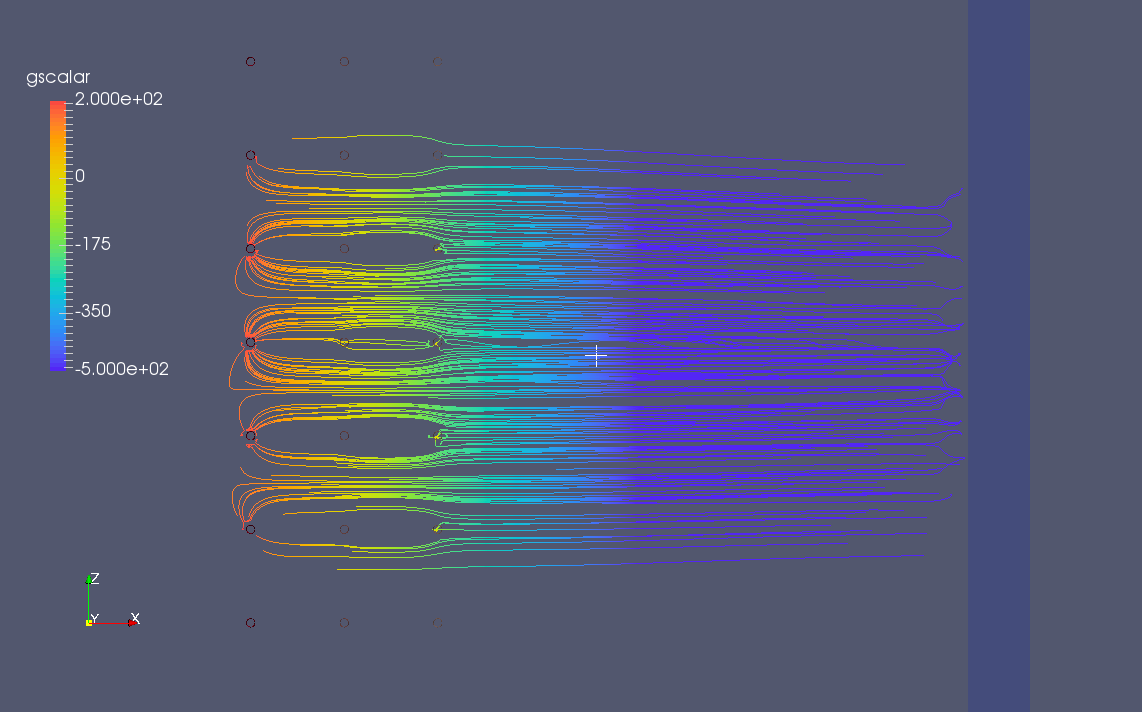
\includegraphics[width=\textwidth]{twodee-fine-steps-plan-gradfixed.png}      
    \end{column}
    \begin{column}{0.5\textwidth}
      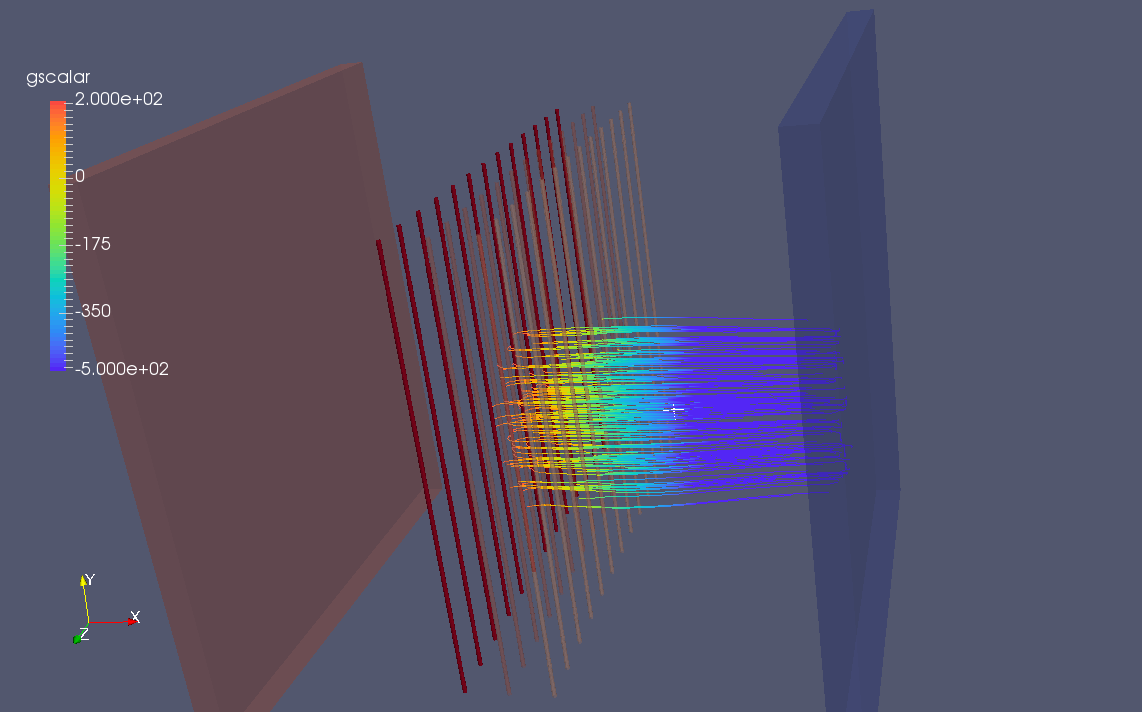
\includegraphics[width=\textwidth]{twodee-fine-steps-side-gradfixed.png}      
    \end{column}
  \end{columns}
  \footnotesize
  \begin{itemize}
  \item The steps no longer go wild high/low.
  \end{itemize}
\end{frame}

\end{document}